\documentclass[a4paper,11pt]{jarticle}
% ファイル先頭から\begin{document}までの内容(プレアンブル)については,
% 教員からの指示がない限り, { } の中を書き換えるだけでよい.

% ToDo: 提出要領に従って,適切な余白を設定する
\usepackage[top=25truemm,  bottom=30truemm,
            left=25truemm, right=25truemm]{geometry}

% ToDo: 提出要領に従って,適切なタイトル・サブタイトルを設定する.
\title{情報工学実験Cレポート \\
       クライアントサーバモデルを基にした\\ネットワークプログラミング}

% ToDo: 自分自身の氏名と学生番号に書き換える
\author{氏名: 島谷 隼生 (Shimatani Toshiki) \\
        学生番号: 09428526}

% ToDo: 教員の指示に従って適切に書き換える
\date{出題日: 2018年12月04日 \\
      提出日: 2019年01月29日 \\
      締切日: 2019年01月29日 \\} 

% ToDo: 図を入れる場合,以下の1行を有効にする
\usepackage[dvipdfmx]{graphicx}

\begin{document}
\maketitle

% 目次つきの表紙ページにする場合はコメントを外す
%{\footnotesize \tableofcontents \newpage}

%%%%%%%%%%%%%%%%%%%%%%%%%%%%%%%%%%%%%%%%%%%%%%%%%%%%%%%%%%%%%%%%
\section{クライアントサーバモデルとは}
%%%%%%%%%%%%%%%%%%%%%%%%%%%%%%%%%%%%%%%%%%%%%%%%%%%%%%%%%%%%%%%%
この章では,本実験の最終課題であるクライアントサーバモデルに基づくプログラムの作成にあたって,
基礎となるクライアントサーバモデルの詳細を説明する.

\subsection{クライアントサーバモデルとは}
クライアント・サーバモデルとは,プログラムがそれぞれクライアント,サーバと呼ばれる2つの部分に
機能を分割する,コンピュータネットワークにおけるソフトウェア構造の一つである.
クライアントプログラムでは,他のサーバプログラムから提供されるサービスを使用する機能を,
サーバプログラムでは,クライアントプログラムに対してサービスを提供する機能を持つ.
\subsection{通信の仕組み}
クライアントサーバモデルでは,機能を分割しているため,互いの処理の結果をネットワークを通じて
交換する必要がある.そのため,クライアントプログラムとサーバプログラムでは,
要求メッセージと応答メッセージという形でデータのやりとりを行っている.
今回はTCP/IP通信をメインにプログラムを作成するため,TCP/IPでの送受信関数を利用して
メッセージの交換を実現している.
\subsection{クライアントとサーバのそれぞれにおける処理の流れ}
以下に大まかな処理のフローチャートを示す.
\begin{figure}[htbp]
\begin{center}
\caption{クライアントサーバモデルのフローチャート}
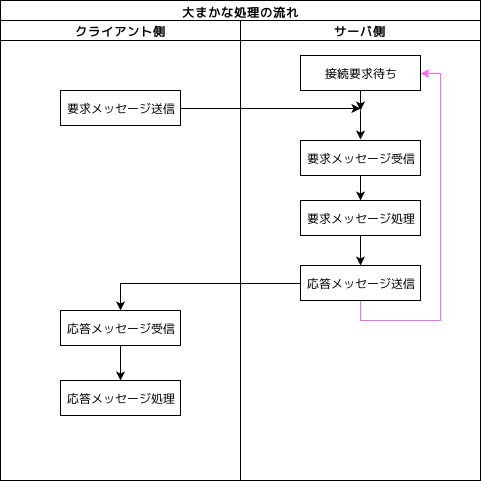
\includegraphics[bb=0 0 481 481, width=7cm]{chart.jpg}

\end{center}
\end{figure}

%%%%%%%%%%%%%%%%%%%%%%%%%%%%%%%%%%%%%%%%%%%%%%%%%%%%%%%%%%%%%%%%
\section{プログラムの作成方針}
%%%%%%%%%%%%%%%%%%%%%%%%%%%%%%%%%%%%%%%%%%%%%%%%%%%%%%%%%%%%%%%%

クライアントプログラムとサーバプログラムのそれぞれにおける作成方針を以下に示す.
また作成にあたり使用していたフローチャートをこの章の最後に示す.

\subsection{クライアントプログラム}
クライアントプログラムは,おおよそ以下の部分から構成することにした.
それぞれについて作成方針を立てる.
\begin{enumerate}
\setlength{\parskip}{2pt} \setlength{\itemsep}{2pt}
    \item プロセス間通信の前処理部(2.1.1項)
    \item 要求メッセージ送信部(2.1.2項)
    \item 応答メッセージ受信部(2.1.3項)
    \item クライアント側コマンド処理部(2.1.4項)
\end{enumerate}


%--------------------------------------------------------------%
\subsubsection{プロセス間通信の前処理部} \label{sec:pre}
%--------------------------------------------------------------%

クライアントプログラムでの``プロセス間通信の前処理部''はクライアントサーバ間でメッセージのやりとりを行うにあたり
必要な処理を行う部分である.
TCP/IPを利用した通信で,
クライアントがメッセージを送信するためには,まずメッセージの送り先を得る必要がある(getbyname).
その後,サーバとのデータ交換口を作成(socket)し,サーバと接続を確立(connect)する.
ここまでがクライアントサーバ間でのメッセージ交換に必要な前処理である.

TCP/IPを利用する場合,socket関数を使用する際に,第一引数,第二引数にそれぞれ
AF\_INET, SOCK\_STREAMを指定する.UDPを利用したい場合は,socket関数の第二引数を
SOCK\_DGRAMに変更する必要がある.


%--------------------------------------------------------------%
\subsubsection{要求メッセージ送信部} \label{sec:send}
%--------------------------------------------------------------%

``要求メッセージ送信部''は標準入力から得られた入力をサーバに送信する部分である.
基本的には入力されたデータをそのまま送信すればよい.だがサーバ側でどのようにメッセージを
読み取るのかを意識する必要がある.今回はサーバ側で一文毎にメッセージの処理を行うようにしているおり,
一文の定義を改行コードがくるまでとしているため,メッセージ送信の場合に必ず終端に改行コードが
ある必要がある.

また,クライアント側で実行する操作がある場合にはこの段階で分岐し,
コマンド処理部に処理を渡すことを推定する
(具体的には\%Qコマンドなど).

%--------------------------------------------------------------%
\subsubsection{応答メッセージ受信部} \label{sec:recv}
%--------------------------------------------------------------%

``応答メッセージ受信部''はサーバから送られてきた,要求メッセージを処理した結果を受け取る
部分である.基本的に受け取ったメッセージは標準出力に出力するのみであると想定する.
しかしサーバ側が複数回にわけて応答メッセージを送信する場合はクライアントとサーバ間で同期をとる必要性が考えられる.


%--------------------------------------------------------------%
\subsubsection{クライアント側コマンド処理部} \label{sec:command}
%--------------------------------------------------------------%

``クライアント側コマンド処理部''はクライアント側で行う必要があるコマンドに対応する処理を行う部分である.
具体的にはクライアントプログラムを終了する\%Qコマンドやクライアントプログラムを起動した計算機にあるファイルを
読み込むための\%Rコマンド等が想定される.

大まかな挙動は以前の実験で作成した名簿管理プログラムと共通するが,ネットワークプログラムとしていくつか変更する
必要がある.例えば\%Qコマンドでは,元はexit関数を使用するだけだったが,今回はソケットをクローズする処理を
追加しなければならない.


\subsection{サーバプログラム}
サーバプログラムは,おおよそ以下の部分から構成することにした.
それぞれについて作成方針を立てる.
\begin{enumerate}
\setlength{\parskip}{2pt} \setlength{\itemsep}{2pt}
    \item プロセス間通信の前処理部(2.2.1項)
    \item 要求メッセージ受信部(2.2.2項)
    \item メッセージ処理部 (2.2.3項)
    \item 応答メッセージ送信部(2.2.4項)
    \item サーバ側コマンド処理部(2.2.5項)
\end{enumerate}


%--------------------------------------------------------------%
\subsubsection{プロセス間通信の前処理部} \label{sec:pre}
%--------------------------------------------------------------%

サーバプログラムでの``プロセス間通信の前処理部''はクライアントサーバ間でメッセージのやりとりを行うにあたり
必要な処理を行う部分である.
クライアントとのデータの交換口を作成(socket)する点ではクライアント側と処理は共通するが,その他は大きく異なる.
サーバプログラムでは,ソケットを作成したのちにソケットに名前付け(bind)を行い,名付けしたソケットを接続待ち状態
にする(listen)必要がある.そして接続待ちとなったソケットに接続しようとしてきたクライアントを
受け入れる(accept)ことでサーバプログラムの前処理は終了する.

クライアント側と同様に,TCP/IPを利用する場合,socket関数を使用する際に,第一引数,第二引数にそれぞれ
AF\_INET, SOCK\_STREAMを指定する.UDPを利用したい場合は,socket関数の第二引数を
SOCK\_DGRAMに変更する必要がある.

また,bind関数で使用するsockaddr構造体のメンバ,sin\_addr構造体のメンバs\_addrに任意のアドレスを意味する
INADDR\_ANYをhtonl関数を使用して設定しておくことに注意する.この操作により,接続を受け付けるソケットは任意の計算機
からアクセスを受け付けることができる.INADDR\_BROADCASTを設定しても
同様の効果が得られるようだが,詳細な理由は分からなかった.

accept関数を使用する際には,引数となるソケットと返り値となるソケットが別となることに注意する.
サーバ処理メインルーチンでは返り値となるソケットを用いてクライアントと通信を行う.

%--------------------------------------------------------------%
\subsubsection{要求メッセージ受信部} \label{sec:send}
%--------------------------------------------------------------%

``要求メッセージ受信部''ではクライアントから送信されてきたメッセージを受信する部分である.
クライアント側から改行文字を区切りとする1行メッセージが送信される想定であるから,これを
処理しやすい形に変える簡単な処理を加える.具体的にはメッセージの改行文字をナル文字の置き換えする処理である.
この処理により配列処理の関数が適用できるようになり,以前作成した名簿管理プログラムの大枠を流用できると考える,

置換処理を加えた後,メッセージを``メッセージ処理部''に渡すことで,この部分の処理は終了する.

作成中は,受信したメッセージをサーバ側の標準出力に出力させることでエラーの有無を確認することを想定する.
%--------------------------------------------------------------%
\subsubsection{メッセージ処理部} \label{sec:send}
%--------------------------------------------------------------%
``メッセージ処理部''は``要求メッセージ処理部''で処理しやすい形に変更されたメッセージを
以前作成した名簿管理プログラムで処理を行う部分である.多くの処理が流用できると考えているが,
結果の出力部分はsend関数を用いてクライアント側に送信しなければならないので,多少の修正が
必要である.

名簿データの登録はこの部分で行うことを想定するが,コマンド処理は``サーバ側コマンド処理部''に
処理を委ねることを想定する.処理部を分割して作成することで,機能拡張が容易になると考えられる.

%--------------------------------------------------------------%
\subsubsection{応答メッセージ送信部} \label{sec:recv}
%--------------------------------------------------------------%

``応答メッセージ送信部''は``メッセージ処理部'',``サーバ側コマンド処理部''で処理された結果を
クライアント側に送信する部分である.基本的に処理内容をソケットに出力するのみであると想定する.

2.1.3項でも述べたが,応答メッセージを繰り返して出力する必要がある場合(\%Pコマンド等)は,
クライアント側と同期を取る必要があると考えられる.

%--------------------------------------------------------------%
\subsubsection{サーバ側コマンド処理部} \label{sec:command}
%--------------------------------------------------------------%

``サーバ側コマンド処理部''は
サーバ側で行う必要があるコマンドに対応する処理を行う部分である.
具体的にはサーバ側に保存してある名簿データに関する情報を提供する\%Pコマンドや\%Cコマンド,
ファイルに名簿データを書き込む\%Wコマンドが考えられる.

それぞれを関数として実装し,``メッセージ処理部''から処理を受け取れるようにする.

\%Pコマンド実装に渡り,名簿データをバッファリングし,通信処理回数を減らすことも考えられる.
時間があれば実装することを考える.時間がない場合は,データを一つ一つ送信する仕様とする.


\%Qコマンドに関しては,クライアントとの接続の終了処理のみにとどめ,サーバプログラム自体は終了しないように
注意する.終了してしまうと,次のクライアントからの接続に応えられなくなるためである.

%--------------------------------------------------------------%
\subsection{作成にあたり使用したフローチャート} \label{sec:command}
%--------------------------------------------------------------%
図2は作成にとりかかるに当たって使用したフローチャートである.完成した名簿管理プログラムと
完全に一致する訳ではないが,大まかな流れと一致するため,ここに示しておく.

\begin{figure}[htbp]
\begin{center}
\caption{クライアントサーバモデルの名簿管理プログラムのフローチャート}
\includegraphics[bb=0 0 771 1031, scale=0.4]{flow.jpg}

\end{center}
\end{figure}
%%%%%%%%%%%%%%%%%%%%%%%%%%%%%%%%%%%%%%%%%%%%%%%%%%%%%%%%%%%%%%%%
\section{プログラムおよびその説明}
%%%%%%%%%%%%%%%%%%%%%%%%%%%%%%%%%%%%%%%%%%%%%%%%%%%%%%%%%%%%%%%%

プログラムリストは$7$章に添付している.クライアントプログラムとサーバプログラムは,それぞれ$xx$行, 
$yy$行からなる.
作成を進めていく過程で作成方針で大まかに分類した構成要素が統合した部分があるため,
実際のプログラムの流れにしたがいながら,作成方針から修正を加えた点などを示す.

また,クライアントサーバ間でのプロトコルについてもここで説明する.

%--------------------------------------------------------------%
\subsection{クライアントプログラム}
%--------------------------------------------------------------%
%--------------------------------------------------------------%
\subsubsection{プロセス間通信の前処理部} 
%--------------------------------------------------------------%
この部分では,前章で示したように,サーバと通信するためにgethostbyname,socket,connect関数を順に使用していき,
要求メッセージ送信のための準備を行う.また gethostbyname関数に渡すIPアドレス,またはドメイン名はコマンドライン引数
から渡すように実装したため,プログラム実行時の第一引数にIPアドレスかドメイン名を指定する仕様となっている.
引数が無い場合はエラー出力を行い,プログラムを終了させる.今回は同一計算機内で動作させることが多いため,
多くの場合はコマンドラインからローカルループバックアドレスである``127.0.0.1''を指定する.

概ね方針通りに作成を行ったが,それぞれの関数でエラーが出た場合のエラー処理を加えた.
エラーが出た場合は,途中でプログラムを終了する.
%--------------------------------------------------------------%
\subsubsection{要求メッセージ送信部} 
%--------------------------------------------------------------%
この部分では,前章で示したように標準入力から得られた入力を要求メッセージとして送信する.

ここの部分も概ね方針どおりであり,改行文字が入力されるまでの入力内容を要求メッセージとして送信する.
だが,作成方針でも示したように,入力内容がコマンド(\%から始まる入力)であった場合,
クライアント側で実行するコマンドではないかをチェックし,実行するコマンドであれば処理をコマンド関数に渡す.
ここで,コマンドの内容によっては引数を持つことがあるため,二つの配列(cmd1,cmd2)を用意し,sscanf関数を用いて
入力内容に空白が含まれる場合に分割している.

また,送信するメッセージの終端には必ず改行文字があることを定めているため,仕様に一致するように以下の記述を行っている.
\begin{verbatim}
if((n = read(0, recv_buf, BUFSIZE-1))<= 0) break;
      recv_buf[n]='\n';
\end{verbatim}
この記述により,送信するメッセージの終端には必ず改行文字が設定される.

方針から異なり,加えた点としてselect関数の使用がある.これは標準入力に一定の時間入力がなかった場合,
クライアントプログラムを終了させるために実装した.詳しくは5章にて説明する.これに伴い,応答メッセージ受信部でも
socket関数への対応部分が加えられている.

%--------------------------------------------------------------%
\subsubsection{応答メッセージ受信部} 
%--------------------------------------------------------------%
この部分では,前章で示したようにサーバ側から送信された応答メッセージを受信し,出力する.

方針通りに結果は出力するのみであるが,サーバ側からのメッセージの受信に失敗した場合は,
エラー処理をし,プログラムを終了する. 

前項でも述べたように,select関数への対応がここにも加えられている.詳しくは5章にて説明する.
select関数への対応により,\%Pコマンドに関しては同期をとる必要がなくなった.このことも5章にて説明する.
%--------------------------------------------------------------%
\subsubsection{クライアント側コマンド処理部} 
%--------------------------------------------------------------%
この部分では,前章で示したようにクライアント側で行う必要のあるコマンドを処理する部分である.

作成方針とは異なり,\%Qコマンドはこの部分に記述せず,要求メッセージ送信部のコマンド処理部への分岐処理の際に,
\%Qに相当する処理を組み込んで実装することとした.
これにより\%Qコマンドの機能を果たす関数の作成は行っていない.

\%R,\%Wコマンドは方針どおり関数を作成し,実装を行っている.
前章の応答メッセージ受信部で述べたがメッセージを繰り返し送受信する場合には同期が必要となる.
コマンド処理部ではselect関数の恩恵が得られないため,応答メッセージ受信部とは異なり,同期が必要で,
同期を行わない場合,メッセージが2回以上,すなわち\%R,\%Wコマンドの場合は名簿データが2件以上となる場合,
正しくメッセージをやりとりできなくなる.

同期は次の順に行われていく.
\begin{enumerate}
\setlength{\parskip}{2pt} \setlength{\itemsep}{2pt}
    \item クライアントサーバ間でメッセージを送りあい,互いに準備ができたことを確認する
    \item 送信側がメッセージを送信し,ループを回すことで何かメッセージが送られて来るまで待機する
    \item 受信側はメッセージを受信後,処理を行い,送信側に処理が完了したことを知らせるメッセージを送信する
    \item 送信側がメッセージを受け取ったら2に戻る
\end{enumerate}

\%R,\%Wコマンドに応じて,送信側と受信側がクライアントとサーバで入れ替わっている.
また,名簿データ以外のメッセージは便宜的なものであるため,クライアント,サーバの双方で適当にackという名前で配列を作成し,
利用している.

%--------------------------------------------------------------%
\subsection{サーバプログラム}
%--------------------------------------------------------------%
%--------------------------------------------------------------%
\subsubsection{プロセス間通信の前処理部} \label{sec:pre}
%--------------------------------------------------------------%
この部分では,前章で示したように,クライアントと通信するためにsocket,bind,listen,accept関数を順に使用していき,
要求メッセージ受信のための準備を行う.クライアント側と同様に,概ね方針どおりに作成したが,
それぞれの関数に対するエラー処理は加えている.エラー処理がでた場合はプログラムが終了するしようとなっている.
%--------------------------------------------------------------%
\subsubsection{要求メッセージ受信部} \label{sec:pre}
%--------------------------------------------------------------%
この部分では,前章で示したように受け取った要求メッセージの末尾を置換する部分である.
以下の様な実装を行っている.
\begin{verbatim}
	receive: /* ストリーム型のデータの受信処理 */  
	  if(rn = recv(new_s,&recv_buf[i],1,0) < 0) break;
	  /* 改行単位で受信処理をする */
	  if (recv_buf[i] != '\n') {
	    i++;
	    if (i < BUFSIZE - 1)
	      goto receive;
	  }
	  recv_buf[i] = '\0';
                       :
          if((recv_msg_exe(recv_buf, new_s))<=0) break;
\end{verbatim}
ソケットに送られたメッセージを一文字ずつ読み取り,改行コードが現れれば末尾をナル文字に置き換え,
メッセージ処理部に渡している.メッセージが指定のバッファサイズを超えるようであれば,
途中で読み取りを終了し,末端にナル文字を置き,メッセージ処理部に渡している.
この仕様により,名簿データの任意長であるコメント部がバッファサイズに制限されることとなっている.
%--------------------------------------------------------------%
\subsubsection{メッセージ処理部} \label{sec:pre}
%--------------------------------------------------------------%
この部分では,前章で示したように,末尾が置換されたメッセージを以前作成した名簿管理プログラムで処理を行う部分である.
それぞれのコマンド関数にソケットを渡す点と,名簿データの入力値が不正だった場合に標準エラー出力に出力していた
エラーメッセージを応答メッセージをする点を除けば,ほとんどを流用することができた.
%--------------------------------------------------------------%
\subsubsection{応答メッセージ送信部} \label{sec:pre}
%--------------------------------------------------------------%
この部分が最も作成方針からはずれた部分である.作成方針では独立した部分であったが,実際に作成にあたり,
名簿データの登録の際は応答メッセージを返す必要がないため,コマンド処理部に応答メッセージの送信を
委ねると独立して作成する必要性が低くなった.作成したプログラムで応答メッセージ送信部にあたる部分は
それぞれコマンド関数内部に含まれるか,元の名簿管理プログラムでのデータ登録の際のエラー出力の部分に
統合した.

%--------------------------------------------------------------%
\subsubsection{サーバ側コマンド処理部} \label{sec:pre}
%--------------------------------------------------------------%
この部分では,前章で示したようにサーバ側で行う必要のあるコマンドを処理する部分である.

この部分で実装したのは,\%C,\%Pコマンドを実装した.%およびサーバ側のファイルを指定する\%R,\%Wコマンドと
%同様の機能を果たす\%SR,\%SWコマンドを実装した.またサーバ側のファイルを指定するにあたり,
%サーバ側にどのようなファイルがあるか分からなければ不便であると考えたため,popen関数を利用して
%サーバ側の特定のファイルの中身を出力させる\%LSコマンドを実装した.

\%Pコマンド関数に関しては,元から作成してあった名簿データを出力するprint\_profile関数の出力先を
標準出力から送信バッファに変更することで実現した.

\%Cコマンドも結果の出力先を標準出力から送信バッファに変更することで実現した.
%--------------------------------------------------------------%
\subsection{クライアントサーバ間でのプロトコル }
%--------------------------------------------------------------%
ここではクライアントサーバ間でのプロトコルを示す.
要求メッセージと応答メッセージの末尾には必ず改行文字がなければならない.
この処理はユーザは特に意識する必要はないが,読み込むCSVファイルを作成する際に,
改行区切りの1行ずつに一つの名簿データのみ読み取ることに注意する.
また以下の表では各コマンドとそのコマンド実行時の返り値を示す.

\begin{table}[b] % 表の位置は原則として t または b である.hやHは使わない.
    \centering % この1行はbegin〜endの中を中央寄せにする,というコマンド
    \caption{実装したコマンド}
    \label{tbl:commands}
    \begin{tabular}{|l|l|l|}
        \hline
        コマンド & 意味 & 返り値\\
        \hline
        \verb|%Q(q)| & プログラムの終了(\verb|Quit|) & なし\\
        \hline
        \verb|%C(c)| & 登録項目数の出力(\verb|Check|) & int型で現在のデータ登録数\\
        \hline
        \verb|%P(p) n| & \verb|CSV| の先頭から\verb|n|番目を抜き出して表示(\verb|Print|) & char型の配列で表の上の形式のバッファ\\
        \hline
        \verb|%R(r) file| & \verb|file|から読込み(\verb|Read|) & 成功時はOKの文字列,失敗時はエラーメッセージ\\
        \hline
        \verb|%W(w) file| & \verb|file|から書出し(\verb|Write|) & 成功時はOKの文字列,失敗時はエラーメッセージ\\
        \hline
    \end{tabular}
\end{table}

{\fontsize{10pt}{11pt} \selectfont
\begin{verbatim}
        Id    : 8681139
        Name  : Cedars School of Excellence
        Birth : 1967-11-03
        Addr  : Lothian Road Greenock
        Com.  : 01475 631074 Primary 20 3.1 Secondary 11 2.6 Ope

\end{verbatim}
}



%%%%%%%%%%%%%%%%%%%%%%%%%%%%%%%%%%%%%%%%%%%%%%%%%%%%%%%%%%%%%%%%
\section{プログラムの使用法}
%%%%%%%%%%%%%%%%%%%%%%%%%%%%%%%%%%%%%%%%%%%%%%%%%%%%%%%%%%%%%%%%

本プログラムは名簿データを管理するためのプログラムである.
クライアント側でCSV形式のデータと \% で始まるコマンドを標準入力から受け付け,サーバに送信し,
サーバ側で受信した内容を処理し,その結果をクライアントに送信する.

プログラムは,一般的な UNIX で用いることを意図している 
\verb|gcc|でコンパイルした後,プログラムを実行する.
その際,サーバを先に実行することと,クライアントではコマンドライン引数でIPアドレスまたはドメイン名が
必要であることに注意する.

プログラム実行後,手入力でCSV形式でデータを入力するか,各種コマンドを使用する.

{\fontsize{10pt}{11pt} \selectfont
 \begin{verbatim}
   \$ gcc -o server server.c
   \$ ./server

   \$ gcc -o client client.c
   \$ ./client 127.0.0.1
   \$ 09428900,Takahashi Kazuyuki,1977-04-27,3,Saitama,male
   \$ %C
 \end{verbatim}
}

プログラムの出力結果としてはCSVデータの各項目を読みやすい形式で出力する.
例えば,下記の sample.csv に対して,

{\fontsize{10pt}{11pt} \selectfont
 \begin{verbatim}
< 09428900,Takahashi Kazuyuki,1977-04-27,Saitama,male
< 09428901,Honma Mitsuru,1972-08-25,Hokkaidou,male
< %C
< %P
< %P 1
< %Q
 \end{verbatim}
}

\noindent 
以下のような出力を得る.

{\fontsize{10pt}{11pt} \selectfont
 \begin{verbatim}
> 2 profile(s)
   
Id    : 9428590
Name  : Takahashi Kazuyuki
Birth : 1977-04-27
Addr  : Saitama
Com.  : male

Id    : 94285901
Name  : Honma Mitsuru
Birth : 1972-08-25
Addr  : Hokkaido
Com.  : male
  
Id    : 94285900
Name  : Takahashi Kazuyuki
Birth : 1977-04-27
Addr  : Saitama
Com.  : male

> Bye.
 \end{verbatim}
}

\noindent
入力された
\verb|%C|は,これまでの入力データが
何件登録されたかということを示し,
\verb|%P| は 入力したデータを全件表示することを
示している.また,
\verb|%P 1|は入力したデータを先頭から
1件(負の数だと後ろから)表示することを示し,
\verb|%Q|はプログラムを終了することを示す.

上の例では\verb|%Q|,\verb|%C|,\verb|%P|コマンドの説明を行った.
以下では残りの\verb|%R|,\verb|%W|コマンドの説明を行う.
\verb|%R|,\verb|%W|コマンドを使用すると,以下のようなsample.csvに対して,

{\fontsize{10pt}{11pt} \selectfont
 \begin{verbatim}
(sample.csv)
   09428900,Takahashi Kazuyuki,1977-04-27,Saitama,male
   09428901,Honma Mitsuru,1972-08-25,Hokkaidou,male
   09428902,Nakamura Hiroki,1975-09-04,Nagano,male
  \end{verbatim}
}
\noindent
次のような応答が得られる.
{\fontsize{10pt}{11pt} \selectfont
 \begin{verbatim}
< %R sample.csv
looding ...
OK.
< %W a.csv
OK.
< %C
> 3 profile(s)
< %P
Id    : 94285900
Name  : Takahashi Kazuyuki
Birth : 1977-04-27
Addr  : Saitama
Com.  : male  

Id    : 94285901
Name  : Honma Mitsuru
Birth : 1972-08-25
Addr  : Hokkaido
Com.  : male

Id    : 94285902
Name  : Nakamura Hiroki
Birth : 1975-09-04
Addr  : Nagano
Com.  : male 
 \end{verbatim}
}
\noindent
出力後,a.csvは以下のように書き換えられている.

{\fontsize{10pt}{11pt} \selectfont
 \begin{verbatim}
   09428900,Takahashi Kazuyuki,1977-04-27,Saitama,male
   09428901,Honma Mitsuru,1972-08-25,Hokkaidou,male
   09428902,Nakamura Hiroki,1975-09-04,Nagano,male
  \end{verbatim}
}
\noindent


%%%%%%%%%%%%%%%%%%%%%%%%%%%%%%%%%%%%%%%%%%%%%%%%%%%%%%%%%%%%%%%%
\section{作成過程における考察}
%%%%%%%%%%%%%%%%%%%%%%%%%%%%%%%%%%%%%%%%%%%%%%%%%%%%%%%%%%%%%%%%
本章では,名簿管理プログラムの作成過程において検討した内容,工夫した内容,
および,考察した内容について述べる.

%--------------------------------------------------------------%
\subsection{\%R,\%Wコマンドの考察}
%--------------------------------------------------------------%
ここでは,\%Rと\%Wコマンドに関して,クライアント側かサーバ側かのどちらのファイルを指定するかを考察する.
この2つをそれぞれ考えていく.

\%Rコマンドに関しては,まずその使い道を考えると,クライアント側のファイルを指定する場合では
クライアント側が保持するCSV形式の名簿データをまとめて登録したい場合に使用することが考えられ,
サーバ側のファイルを指定する場合は\%Wをサーバ側のファイルを指定するとした場合に,
データを取り出す役割を果たす.

\%Wコマンドに関しては,同様に使い道を考えると,クライアント側でファイルを指定する場合は名簿データをクライアント側が
手元に残したい場合に使用することが考えられる.サーバ側でのファイルを指定する場合は現在登録されているデータを
一時退避させる際に使用することが考えられる.そうすることでクライアントが終了した後,再接続した際に同じデータを
自動で読み取る機能の実装等に使用できる.

これらを踏まえとどちらの実装でもメリットは存在するといえる.
そこで,次にクライアントサーバモデルの名簿管理プログラムという意味を考えていく.
クライアントサーバモデルである以上,サーバ側の負担はできる限り少ないほうがよいと考える.
つまり複数のクライアントに利用されることを想定するのであれば,サーバ側にデータを保存すると
サーバ側に多くの名簿データが記憶され,場合によっては他のクライアントにデータを書き換えられる可能性がある.
そのためクライアント側で\%R,\%Wコマンドを実装するべきと考える.


%--------------------------------------------------------------%
\subsection{サーバ側の多重受付に関する考察}
%--------------------------------------------------------------%
当初の作成方針では,サーバは1つのクライアントとしか通信できず,現実的なプログラムではなかった.
そのため,多数のクライアントから同時に要求を受け付けられるように拡張することを考えた.
考えられる手法は,select関数を用いる方法と,fork関数を用いる方法である.
今回採用した方法はfork関数である.理由は2点あり,select関数とfork関数のクライアントの上限を考えた場合,
select関数はファイルディスクプタの上限数であり,fork関数はサーバ側が同時に起動できるプロセスの最大数であるため,
fork関数の方がより多くのクライアントに対応できると考えた点と,fork関数で実装するとプログラムを再帰的に実行させることで
簡単に実現できる点である.この2点の理由によりfork関数を用いる手法を採用した.

この結果,サーバ側の多重受付が可能となった.


%--------------------------------------------------------------%
\subsection{select関数の使用}
%--------------------------------------------------------------%
今回,クライアントプログラムで作成方針と異なった点としてselect関数の使用が挙げられる.
select関数は登録したソケットを監視し,データが受信可能となったソケットにread関数等を使用できるようにする関数である.
これを実装することで,クライアントプログラムのメインルーチンを標準入力とサーバーと接続されたソケット部に分割
することができ,サーバが連続してソケットにメッセージを送っても逐一同期をとる必要がなくなった.これは
クライアントがコマンドを実行したあと,サーバが繰り返しメッセージを送信しても,クライアントは受信したメッセージを
処理した後,再びデータを受信しているソケットを読み込むためである.

しかし,これはselect関数のループ内に限ってである.\%Rや\%Wコマンドでコマンド関数内部で処理を行う際は,
一つのソケットしかなく,入出力口が共有されているため同期が必要となる.
%%%%%%%%%%%%%%%%%%%%%%%%%%%%%%%%%%%%%%%%%%%%%%%%%%%%%%%%%%%%%%%
\section{結果に関する考察}
%%%%%%%%%%%%%%%%%%%%%%%%%%%%%%%%%%%%%%%%%%%%%%%%%%%%%%%%%%%%%%%%
ここでは,以下の項目について考察を述べる.

\begin{enumerate}
\setlength{\parskip}{2pt} \setlength{\itemsep}{2pt}
    \item 不足機能についての考察
    \item ゾンビプロセスについての考察
    \item クライアントサーバモデルによる機能の制限
\end{enumerate}

%--------------------------------------------------------------%
\subsection{不足機能についての考察}
%--------------------------------------------------------------%

考えられる不足機能としては,登録されたデータをリセットし0件とする\verb|%reset|コマンド,
採用しなかったサーバ側のファイルを使用する\%R,\%Wコマンド,
実装してあるコマンドを説明する機能などが考えられる.
それぞれの理由を説明する.まず,登録されたデータをリセットし0件とする\verb|%reset|コマンドについてだが,
データが10000件に達するともとの名簿管理プログラムの仕様上データの登録が出来無い.登録データを\%Wコマンドで
書き込みした後,リセットできなければ逐一クライアントプログラムを終了する必要がある.
次に,採用しなかったサーバ側のファイルを使用する\%R,\%Wコマンドであるが,このコマンドは名簿データの共有が
異なるクライアント間でできるため採用の価値があるが,\%Rコマンドがうまく実装できなかったため断念した.
実装してあるコマンドを説明する機能は,いわゆるヘルプ機能である.プログラムを用いる人がプログラムの使用方法を完全に知っている
可能性は高くないため,それを補う必要がある.そのための機能である.

%--------------------------------------------------------------%
\subsection{ゾンビプロセスについての考察}
%--------------------------------------------------------------%
前章で,fork関数を利用してサーバ側の多重要求受付を実現したことを述べた.
このfork関数にはゾンビプロセスと呼ばれる問題が存在する.
fork関数の機能は子プロセスを生成するというものでる.生成された子プロセスが終了した際に
親プロセスがwait関数を用いて子プロセスの終了を確認する必要があるが,子プロセスの終了前に,
親プロセスが終了してしまうと,子プロセスの終了確認ができず,プロセステーブルに残り続けるという
現象が生じる.しかしwait関数の使用中は親プロセスの処理が停止するため,名簿管理プログラムがうまくいかない.
解決方法を模索したが,時間が足りず解決には至らなかった.

%--------------------------------------------------------------%
\subsection{クライアントサーバモデルによる機能の制限}
%--------------------------------------------------------------%
今回,名簿管理プログラムをクライアントサーバモデルに対応させたことにより,本来の仕様に制限がかかった部分がある.
具体的には任意長のコメント部分である.
プロセス間通信にsendやrecv関数を用いるため,今回送信バッファと受信バッファを設定し,バッファサイズをマクロ定義で
定めているため,定義したバッファサイズまでしかコメントを書くことができなくなってしまっている.
この対策として,バッファ長以上にコメントが伸びている場合に,分割して送信することで任意長を維持できると考えたが,
実装する時間がなかったため今回は実装を見送った.

%%%%%%%%%%%%%%%%%%%%%%%%%%%%%%%%%%%%%%%%%%%%%%%%%%%%%%%%%%%%%%%%
\section{作成したプログラム}
%%%%%%%%%%%%%%%%%%%%%%%%%%%%%%%%%%%%%%%%%%%%%%%%%%%%%%%%%%%%%%%%

作成したプログラムを以下に添付する.
\subsection{クライアントプログラム}
{\fontsize{10pt}{11pt} \selectfont
\begin{verbatim}
     1	#include<sys/types.h>
     2	#include<sys/socket.h>
     3	#include<netinet/in.h>
     4	#include<stdio.h>
     5	#include<netdb.h>
     6	#include<string.h>
     7	#include<stdlib.h>
     8	#include <arpa/inet.h>
     9	#include <sys/time.h>
    10	#include <netinet/in.h>
    11	
    12	#define PORT_NO 2018
    13	#define BUFSIZE 1024+1
    14	#define MAX_LINE_LEN 1024 /*1行に読み込める最大文字数*/
    15	
    16	void cmd_read(char *file, int socket);
    17	void cmd_write(char *file, int socket);
    18	
    19	int main(int argc, char* argv[]){
    20	  int s, i=0, len, size, n;
    21	  char recv_buf[BUFSIZE]={0};  /* 受信バッファ                  */
    22	  char send_buf[BUFSIZE]={0};  /* 送信バッファ                  */
    23	  char cmd1[BUFSIZE]={0};
    24	  char cmd2[BUFSIZE]={0};
    25	  struct sockaddr_in sa;
    26	  struct hostent *hp;   
    27	  struct timeval tv;    /* selectのタイムアウト時間       */
    28	  fd_set readfd;        /* selectで検出するディスクリプタ  */
    29	  int cnt;
    30	  if(argc < 2){
    31	    fprintf(stderr,"Error: Didn't set IP_addr or domain\n");
    32	    exit(1);
    33	  }
    34	  if((hp = gethostbyname(argv[1]))==0){
    35	    fprintf(stderr,"Error: Unknwon host.\n");
    36	    exit(1);
    37	  }
    38	
    39	  sa.sin_family = AF_INET;
    40	  sa.sin_port = htons(PORT_NO);
    41	  
    42	  bzero((char *)&sa.sin_addr, sizeof(sa.sin_addr));
    43	  
    44	  memcpy((char *)&sa.sin_addr,(char *)hp->h_addr,hp->h_length);
    45	
    46	  if((s = socket(AF_INET, SOCK_STREAM, 0))==-1){
    47	    fprintf(stderr,"Error: Can't open socket.\n");
    48	    exit(1);
    49	  }
    50	  if(connect(s, (struct sockaddr*)&sa, sizeof(struct sockaddr_in))==-1){
    51	    fprintf(stderr,"Error: Can't connect socket with host.\n");
    52	    exit(1);
    53	  }
    54	
    55	  printf("connected to '%s'\n", inet_ntoa(sa.sin_addr));
    56	
    57	  /* client processing routine */
    58	  while(1){
    59	    //bzero(send_buf,strlen(send_buf));
    60	    //bzero(recv_buf,strlen(recv_buf));
    61	    tv.tv_sec = 600;
    62	    tv.tv_usec = 0;
    63	
    64	    FD_ZERO(&readfd);
    65	    FD_SET(0,&readfd);
    66	    FD_SET(s,&readfd);
    67	    if((select(s+1, &readfd, NULL, NULL, &tv))<=0){
    68	      fprintf(stderr, "\nTimeout\n");
    69	      break;
    70	    }
    71	
    72	    /* standard input */
    73	    if(FD_ISSET(0, &readfd)){
    74	      bzero(cmd1,BUFSIZE);
    75	      bzero(cmd2,BUFSIZE);
    76	      if((n = read(0, recv_buf, BUFSIZE-1))<= 0) break;
    77	      recv_buf[n]='\n';
    78	      cnt = sscanf(recv_buf, "%s%s", cmd1,cmd2);
    79	      if(strcmp(cmd1, "%Q") == 0 ||
    80		 strcmp(cmd1, "%q") == 0) {
    81		printf("Bye.\n");
    82		break;
    83	      }
    84	      if(strcmp(cmd1,"%W")== 0 ||
    85		 strcmp(cmd1,"w") == 0){
    86		send(s,"%W\n",3,0);
    87		if(cnt == 2) cmd_write(cmd2, s);
    88		else if(cnt == 1){
    89		  fprintf(stderr,"%W(%w) command need argument(filename).\n");
    90		  fprintf(stderr,"format: %W (file name)\n");
    91		}
    92		continue;
    93	      }
    94	      if(strcmp(cmd1, "%R") == 0 ||
    95		 strcmp(cmd1, "%r") == 0) {
    96		send(s,"%R\n",3,0);
    97		if(cnt == 2) cmd_read(cmd2, s);
    98		else if(cnt == 1){
    99		  fprintf(stderr,"%R(%r) command need argument(filename).\n");
   100		  fprintf(stderr,"format: %R (file name)\n");
   101		}
   102		
   103		  continue;
   104	      }
   105	      if(send(s, recv_buf, n, 0) <= 0) break;
   106	    }
   107	
   108	    /* server */
   109	    if (FD_ISSET(s, &readfd)){
   110	      //recv(s,recv_buf,2,0);
   111	      //printf("%s",recv_buf);
   112	      //bzero(recv_buf,BUFSIZE);
   113	      if ((n = recv(s, recv_buf, (BUFSIZE)-1, 0)) < 0){
   114		fprintf(stderr, "Error: connection closed. \n");
   115		close(s);
   116		exit(EXIT_FAILURE);
   117	      }
   118	      recv_buf[n]='\0';
   119	      printf("%s",recv_buf);
   120	      fflush(stdout);
   121	    }
   122	  }
   123	  bzero(send_buf, BUFSIZE);
   124	  strncpy(send_buf, "%Q", 2);
   125	  send(s, send_buf, n, 0);
   126	  close(s);
   127	
   128	  return EXIT_SUCCESS;
   129	}
   130	
   131	
   132	/*
   133	  while(1){
   134	    bzero(buf2, sizeof(buf2));
   135	    recv(s,buf2,5,0);
   136	    printf("%s",buf2);
   137	    bzero(buf2, sizeof(buf2));
   138	    scanf("%[^\n]",&buf2);
   139	    i=send(s, buf2, strlen(buf2)+1, 0);
   140	    if(i==-1){
   141	      close(s);
   142	      fprintf(stderr,"Error: Failed sending message.\n");
   143	      exit(1);
   144	    }
   145	    send(s, "\r\n",2,0);
   146	       
   147	    recv(s, buf, strlen(buf2), 0);
   148	    
   149	    printf("%s\n",buf);
   150	  }
   151	}*/
   152	  
   153	void cmd_read(char *file, int socket) {
   154	  FILE *fp;
   155	  char line[BUFSIZE + 1];
   156	  char ack[2]={0};
   157	  int n;
   158	  
   159	  fp = fopen(file, "r");
   160	
   161	  if (fp == NULL) {
   162	    fprintf(stderr,"Could not open file: $s\n", file);
   163	    return;
   164	  }
   165	  
   166	  while(1){
   167	    if((recv(socket,ack,1,0))>0) {
   168	      printf("loading . . .\n");
   169	      break;
   170	    }
   171	    //printf("%d",n);
   172	  }
   173	  while (1) {
   174	    bzero(line,BUFSIZE+1);
   175	    if((fgets(line,BUFSIZE+1,fp)) == NULL) break;
   176	    if(strlen(line) > BUFSIZE) line[BUFSIZE] = '\n';
   177	    send(socket,line,BUFSIZE+1,0);
   178	    while(1){
   179	      if((recv(socket,ack,1,0)) > 0) break;
   180	    }
   181	  }
   182	  printf("OK.\n");
   183	  fclose(fp);
   184	  return;
   185	}  
   186	
   187	void cmd_write(char *file, int socket){
   188	  FILE *fp;
   189	  char line[BUFSIZE + 1];
   190	  char ack[2]={0};
   191	  char recv_buf[BUFSIZE+1]={0};
   192	  int n;
   193	  
   194	  fp = fopen(file, "w");
   195	
   196	  if (fp == NULL) {
   197	    fprintf(stderr,"Could not open file: $s\n", file);
   198	    return;
   199	  }
   200	
   201	  if(strchr(file,'/')!=NULL){
   202	    fprintf(stderr,"This file-name is including invalid character '/' : %s\n", file);
   203	    return;
   204	  }
   205	  while(1){
   206	    if((recv(socket,ack,1,0))>0) {
   207	      break;
   208	    }
   209	  }
   210	  send(socket," ",1,0);
   211	  while (1) {
   212	      bzero(recv_buf,BUFSIZE);
   213	      while(1){
   214		if((recv(socket,recv_buf,BUFSIZE,0)) > 0) break;
   215	      }
   216	      recv_buf[BUFSIZE]='\0';
   217	      if(*recv_buf == '\0') break;
   218	      fprintf(fp,"%s",recv_buf);
   219	      send(socket," ",1,0);
   220	  }
   221	  printf("OK.\n");
   222	  fclose(fp);
   223	  return;
   224	}  
\end{verbatim}
}
 
\end{document}
\subsection{サーバプログラム}
{\fontsize{10pt}{11pt} \selectfont
\begin{verbatim}
     1	#include<sys/types.h>
     2	#include<sys/socket.h>
     3	#include<netinet/in.h>
     4	#include<stdio.h>
     5	#include<netdb.h>
     6	#include<string.h>
     7	#include<stdlib.h>
     8	#include<arpa/inet.h>
     9	#include<sys/time.h>
    10	#include<netinet/in.h>
    11	#include<unistd.h>
    12	
    13	#define PORT_NO 2018
    14	#define BUFSIZE 1024+1
    15	#define MAX_STR_LEN 70 /*構造体メンバnameとhomeの最大文字数*/
    16	#define MAX_SPLIT 5 /*split関数での最大分割数*/
    17	#define PDS profile_data_store
    18	#define PDN profile_data_nitems
    19	
    20	struct date {
    21	  int y;
    22	  int m;
    23	  int d;
    24	};
    25	
    26	struct profile {
    27	  int id;
    28	  char name[MAX_STR_LEN];
    29	  struct date birthday;
    30	  char home[MAX_STR_LEN];
    31	  char *comment;
    32	};
    33	
    34	typedef enum {
    35	  QUITE,
    36	  CHECK,
    37	  PRINT,
    38	  SERVER_WRITE,
    39	  SERVER_READ,
    40	  WRITE,
    41	  READ,
    42	  LINUX_ls,
    43	  LINUX_fd,
    44	  UNKNOWN
    45	} Command;
    46	
    47	struct profile profile_data_store[10000]; /*10000件のデータまで登録可能*/
    48	int profile_data_nitems = 0; /*登録したデータ数*/
    49	int save = 0; /* データを保存したかどうかの判定に使用 */
    50	/*************************************************************************/
    51	void parse_line(char* cmd1, char* cmd2, int socket);
    52	void exec_command(char* cmd1, char* cmd2, int socket);  /* 基本関数 */
    53	void new_profile(char* profile, int socket);
    54	int split(char *str, char *ret[], char sep, int max);
    55	void cmd_quit();                 /************************************/ 
    56	void cmd_check(int socket);
    57	void cmd_print(int n, int socket);
    58	void cmd_read(int socket);
    59	void cmd_write(int socket);
    60	void cmd_serv_read(char *file, int socket);
    61	void cmd_serv_write(char *file, int socket);/*          コマンド関数           */
    62	void cmd_find(char *word);
    63	void cmd_bsort(int n);
    64	void cmd_qsort(int n);
    65	void cmd_modify(int n);
    66	void cmd_delete(int n);
    67	void cmd_find2(char *word);
    68	void cmd_Bwrite(char *line);
    69	void cmd_Bread(char *line);     /************************************/
    70	void cmd_ls(int socket);
    71	void print_profile(struct profile *p, int socket);
    72	void fprint_profile_csv(FILE *fp, struct profile *p);
    73	int execute(char *command, char *buf, int bufmax);
    74	int decide_cmd(char *cmd);
    75	int get_line(FILE *fp,char *line);
    76	int subst(char *str, char c1, char c2);
    77	/*************************************************************************/
    78	
    79	int recv_msg_exe(char* recv_buf, int socket);
    80	
    81	int main(void){
    82	  int s,new_s; /* socket */
    83	  int i; /* loop counter */
    84	  int len,len_c;
    85	  int sn,cn,rn;
    86	  int n;
    87	  int pid; /* fork */
    88	  struct sockaddr_in sa,sa_c;
    89	  char c;
    90	  //char cmd1[BUFSIZE];
    91	  //char cmd2[BUFSIZE];  
    92	  char send_buf[BUFSIZE];
    93	  char recv_buf[BUFSIZE];
    94	  
    95	  if((s = socket(AF_INET, SOCK_STREAM, 0)) < 0){
    96	    fprintf(stderr,"Error: Can't open socket.\n");
    97	    exit(1);
    98	  }
    99	  
   100	  memset((char*)&sa,0,sizeof(sa));
   101	  sa.sin_family = AF_INET;
   102	  sa.sin_port = htons(PORT_NO);
   103	  sa.sin_addr.s_addr=htonl(INADDR_ANY);
   104	
   105	  if(bind(s,(struct sockaddr*)&sa,sizeof(sa)) < 0){
   106	    fprintf(stderr,"Error: Failed Binding stream socket server\n");
   107	    close(s);
   108	    exit(2);
   109	  }
   110	  
   111	  printf("Socket Port %d\n", ntohs(sa.sin_port));
   112	
   113	  if(listen(s,5)==-1){
   114	    fprintf(stderr,"Error: Listen Failed.\n");
   115	    exit(3);
   116	  }
   117	  while(1){ 
   118	    len_c = sizeof(sa_c);
   119	    new_s = accept(s,(struct sockaddr*)&sa_c,&len_c);
   120	    if(new_s==-1){
   121	      fprintf(stderr,"Error: Accept Failed.\n");
   122	      exit(4);
   123	    }
   124	    pid = fork();
   125	    if(pid==0){
   126	      close(s);
   127		/* サーバ処理メインルーチン */
   128		while(1){
   129		  i = 0; /* 受信文字のカウント */
   130		  //bzero(send_buf,strlen(send_buf));
   131		  
   132		  sn = sprintf(send_buf, "< ");
   133		  send(new_s, send_buf, sn, 0);
   134		  
   135		receive: /* ストリーム型のデータの受信処理 */  
   136		  if(rn = recv(new_s,&recv_buf[i],1,0) < 0) break;
   137		  /* 改行単位で受信処理をする */
   138		  if (recv_buf[i] != '\n') {
   139		    i++;
   140		    if (i < BUFSIZE - 1)
   141		      goto receive;
   142		  }
   143		  recv_buf[i] = '\0';
   144		  //printf("receive '%s'\n", recv_buf);
   145		  rn = i;
   146		  //bzero(cmd1,BUFSIZE);
   147		  //bzero(cmd2,BUFSIZE);
   148		  if((recv_msg_exe(recv_buf, new_s))<=0) break;
   149		  bzero(recv_buf,BUFSIZE);
   150		  /* 受信コマンドの処理 */
   151		}
   152	      printf("connection closed.\n");
   153	      //bzero(send_buf,BUFSIZE);
   154	      //bzero(recv_buf,BUFSIZE);
   155	      close(new_s);
   156	      _exit(0);
   157	    }else {
   158	      close(new_s);
   159	    }
   160	  }
   161	  close(s);
   162	  return EXIT_SUCCESS;
   163	}
   164	  
   165	int recv_msg_exe(char* recv_buf, int socket){ 
   166	  int cn;
   167	  char send_buf[BUFSIZE];
   168	  char cmd1[BUFSIZE];
   169	  char cmd2[BUFSIZE];
   170	
   171	  bzero(cmd1,BUFSIZE);
   172	  bzero(cmd2,BUFSIZE);
   173	  bzero(send_buf,BUFSIZE);
   174	
   175	  //if ((cn = sscanf(recv_buf, "%s%s", cmd1, cmd2)) <= 0){
   176	  if (*recv_buf == '%'){
   177	    if ((cn = sscanf(recv_buf, "%s%s", cmd1, cmd2)) <= 0){
   178	      fprintf(stderr,"Input Error\n");
   179	      send(socket, "> Input Error\n",14,0);
   180	      return 2;
   181	    }else if(cn == 1){
   182	      if(strcmp(cmd1, "%Q") == 0) {
   183		printf("exec %Q command.\n");
   184		return 0;
   185		//return 0; /* 0 以下の値を返すと呼び出し側で break文が実行される */
   186	      }else{
   187		*cmd2 = 0;
   188		parse_line(cmd1, cmd2, socket);
   189		return 1;
   190	      }
   191	    }else if(cn == 2){
   192	      parse_line(cmd1, cmd2, socket);
   193	      return 1;
   194	    }
   195	  } else {
   196	    parse_line(recv_buf, NULL, socket);
   197	    return 1;
   198	  }
   199	}
   200	
   201	void parse_line(char* cmd1, char* cmd2, int socket){
   202	    if(*cmd1 == '%'){
   203	      exec_command(cmd1, cmd2, socket);
   204	    }else {
   205	      if (profile_data_nitems < 10000 ) {
   206		new_profile(cmd1, socket);
   207	      }
   208	    }
   209	}
   210	
   211	
   212	void exec_command(char* cmd1, char* cmd2, int socket){
   213	 Command cmd = decide_cmd(cmd1);
   214	    switch(cmd) {
   215	    case CHECK :  cmd_check(socket); break;
   216	    case PRINT : 
   217	      if(cmd2 == NULL) {
   218		cmd_print(0,socket);
   219	      }else{
   220		cmd_print(atoi(cmd2),socket); 
   221	      } break;
   222	    case READ  : cmd_read(socket); break;
   223	    case WRITE : cmd_write(socket); break;
   224	    case SERVER_READ : cmd_serv_read(cmd2,socket); break;
   225	    case SERVER_WRITE :  cmd_serv_write(cmd2, socket); break;
   226	    case LINUX_ls : cmd_ls(socket); break;
   227	    default:
   228	      fprintf(stderr, "%s command is undefined \n", cmd1);
   229	      break;
   230	    }
   231	}
   232	
   233	void new_profile(char* profile, int socket){
   234	  char send_buf[BUFSIZE] = {};
   235	  char *ret[5];
   236	  char *ret2[3];
   237	  int cnt1, cnt2;
   238	  int err_flag = 0;
   239	  
   240	  cnt1 = split(profile, ret, ',', MAX_SPLIT);
   241	  if (cnt1 == 5){
   242	    //printf("%s\n",ret[0]);
   243	    //printf("%s\n",ret[1]);
   244	    //printf("%s\n",ret[2]);
   245	    //printf("%s\n",ret[3]);
   246	    //printf("%s\n",ret[4]);
   247	    if (strlen(ret[0]) > 8) {
   248	      err_flag = 1;
   249	      strcat(send_buf, "> ID max digits are 8.\n");
   250	      //send(socket, send_buf, strlen(send_buf) , 0);
   251	      //fprintf(stderr,"ID max digits are 8\n");
   252	    }
   253	    PDS[PDN].id = atoi(ret[0]);
   254	    strncpy(PDS[PDN].name, ret[1], MAX_STR_LEN);
   255	    PDS[PDN].name[MAX_STR_LEN] = '\0';
   256	    cnt2 = split(ret[2], ret2, '-', 3);
   257	    if (cnt2 == 3) { 
   258	      PDS[PDN].birthday.y = atoi(ret2[0]);
   259	      PDS[PDN].birthday.m = atoi(ret2[1]);
   260	      PDS[PDN].birthday.d = atoi(ret2[2]);
   261	      if (PDS[PDN].birthday.y > 9999 ||
   262		  PDS[PDN].birthday.y < 0    ||
   263		  PDS[PDN].birthday.m > 12   ||
   264		  PDS[PDN].birthday.m < 1    ||
   265		  PDS[PDN].birthday.d < 1    ||
   266		  PDS[PDN].birthday.d > 31) {
   267		if(err_flag == 1) strcat(send_buf, "  ");
   268		else strcat(send_buf,"> ");
   269		err_flag = 1;
   270		strcat(send_buf, "inputed birthday data is inappropriate.\n");
   271		//send(socket, "inputed birthday data is inappropriate.\n", 40,0);
   272		//fprintf(stderr,"inputed birthday data is inappropriate\n");
   273		cnt2 = 0;
   274	      }
   275	    } else if (cnt2 == 2 || cnt2 == 1) {
   276	      if(err_flag == 1) strcat(send_buf, "  ");
   277	      else strcat(send_buf,"> ");
   278	      err_flag = 1;
   279	      strcat(send_buf, "inputed birthday data is inappropriate.\n");
   280	      //send(socket, "inputed birthday data is inappropriate.\n", 40, 0);
   281	      //fprintf(stderr,"inputed birthday data is inappropriate\n");
   282	    } 
   283	    strncpy(PDS[PDN].home, ret[3], MAX_STR_LEN);
   284	    PDS[PDN].home[MAX_STR_LEN] ='\0';
   285	    PDS[PDN].comment = (char*)malloc(sizeof(char*)*(strlen(ret[4])+1));
   286	    ret[4][strlen(ret[4])-1]='\n';
   287	    strcpy(PDS[PDN].comment, ret[4]);
   288	    profile_data_nitems++;
   289	    if (cnt2 != 3 || strlen(ret[0]) > 8) {
   290	      profile_data_nitems--;
   291	      if (cnt2 == 2 || cnt2 == 1 ) {
   292		if(err_flag == 1) strcat(send_buf, "  ");
   293		else strcat(send_buf,"> ");
   294		err_flag = 1;
   295		strcat(send_buf, "correct birtday form example: 2018-01-01\n");
   296	      }
   297	    }
   298	    send(socket, send_buf,strlen(send_buf),0);
   299	  } else {
   300	    strcat(send_buf,"> ");
   301	    strcat(send_buf,"error: this input is wrong form.\n  ");
   302	    strcat(send_buf,"correct form : (ID),(name),(birthday),(home),(comment)\n  ");
   303	    strcat(send_buf,"             : %(command) (argument)\n  ");
   304	    strcat(send_buf,"example: 09428500,Okayama Taro,1998-01-01,okayama,good student\n  ");
   305	    strcat(send_buf,"       : %C\n");
   306	   
   307	    send(socket, send_buf, strlen(send_buf), 0);
   308	      }
   309	}
   310	
   311	int split(char *str, char *ret[], char sep, int max){
   312	  int cnt = 0;
   313	  
   314	  *(ret + (cnt++)) = str;
   315	  
   316	  while (*str && cnt < max) {
   317	    if (*str == sep){
   318	      *str = '\0';
   319	      *(ret + (cnt++)) = str + 1;
   320	    }
   321	    str++; 
   322	  }
   323	  return cnt;
   324	}
   325	
   326	void cmd_check(int socket) {
   327	  char send_buf[BUFSIZE]={0};
   328	  
   329	  sprintf(send_buf,"> %d profile(s)\n",profile_data_nitems);
   330	  send(socket, send_buf, strlen(send_buf),0);
   331	  printf("%d profile(s)\n",profile_data_nitems);
   332	}
   333	
   334	
   335	void cmd_print(int n, int socket) {
   336	  int i;
   337	  if (n > 0) {
   338	    if ( n > profile_data_nitems ) {
   339	      n = profile_data_nitems;
   340	    }
   341	    for( i = 0 ; i < n ; i++) { 
   342	      print_profile(PDS + i, socket);
   343	    }
   344	  } else if (n == 0) {
   345	    for( i = 0 ; i < profile_data_nitems ; i++) { 
   346	      print_profile(PDS + i, socket);
   347	    }
   348	  } else if (n < 0 ) {
   349	    if ( (-1) * n > profile_data_nitems) {
   350	      n = (-1) * profile_data_nitems;
   351	    } 
   352	    for( i = profile_data_nitems + n ; i < profile_data_nitems ; i++) { 
   353	      print_profile(PDS + i, socket);
   354	    }
   355	  }
   356	}
   357	
   358	void print_profile(struct profile *p, int socket) {
   359	  char send_buf[BUFSIZE] = {};
   360	  char tmp_buf[BUFSIZE] = {};
   361	  sprintf(tmp_buf,"Id    : %d\n",p->id);
   362	  strcat(send_buf,tmp_buf);
   363	  bzero(tmp_buf, BUFSIZE);
   364	  sprintf(tmp_buf,"Name  : %s\n",p->name);
   365	  strcat(send_buf,tmp_buf);
   366	  bzero(tmp_buf, BUFSIZE);
   367	  sprintf(tmp_buf,"Birth : %04d-%02d-%02d\n",p->birthday.y,p->birthday.m,p->birthday.d);
   368	  strcat(send_buf,tmp_buf);
   369	  bzero(tmp_buf, BUFSIZE);
   370	  sprintf(tmp_buf,"Addr  : %s\n",p->home);
   371	  strcat(send_buf,tmp_buf);
   372	  bzero(tmp_buf, BUFSIZE);
   373	  sprintf(tmp_buf,"Com.  : %s\n",p->comment);
   374	  strcat(send_buf, tmp_buf);
   375	  send(socket, send_buf, strlen(send_buf), 0);
   376	}
   377	
   378	void cmd_read(int socket){
   379	  char recv_buf[BUFSIZE+1]={0};
   380	  struct timeval tv;
   381	  fd_set readfd;
   382	  tv.tv_sec = 1;
   383	  tv.tv_usec = 0;
   384	  
   385	  FD_ZERO(&readfd);
   386	  FD_SET(socket,&readfd);
   387	
   388	  send(socket," ",1,0);
   389	  
   390	  while(1){
   391	    if((select(socket+1, &readfd, NULL, NULL, &tv))<=0){
   392	      save = 1;
   393	      break;
   394	    }
   395	    recv(socket,recv_buf,BUFSIZE+1,0);
   396	    //if(strcmp(recv_buf,"%Q")==0) break;
   397	    if (profile_data_nitems < 10000 ) {
   398	      new_profile(recv_buf, socket);
   399	    }
   400	    send(socket," ",1,0);
   401	  }
   402	}
   403	
   404	void cmd_write(int socket){
   405	  int i;
   406	  char ack[2]={0};
   407	  FILE *fp,*tmp_fp;
   408	  char tmp_file[22]={"server_file/.tmp.csv"};
   409	  char send_buf[BUFSIZE+1]={0};
   410	
   411	  tmp_fp = fopen(tmp_file,"w");
   412	  for (i = 0; i < profile_data_nitems; i++) {
   413	   fprint_profile_csv(tmp_fp, PDS+i);
   414	  }
   415	  fclose(tmp_fp);
   416	  fp = fopen(tmp_file,"r");
   417	  
   418	  send(socket," ",1,0);
   419	  while(1){
   420	    while(1){
   421	      if(recv(socket,ack,1,0)>0) break;
   422	    }
   423	    if(fgets(send_buf,BUFSIZE+1,fp)==NULL) {
   424	      send(socket,"\0",1,0);
   425	      break;
   426	    }
   427	    send(socket,send_buf,strlen(send_buf),0);
   428	    bzero(send_buf,BUFSIZE);
   429	  }
   430	}
   431	
   432	void cmd_serv_read(char *file, int socket){
   433	  FILE *fp;
   434	  char line[BUFSIZE];
   435	  char filename[BUFSIZE+12]={"server_file/"};
   436	  char send_buf[BUFSIZE]={0};
   437	
   438	  if(strchr(file,'/')!=NULL){
   439	    sprintf(send_buf,"This file-name is including invalid character '/' : %s\n", file);
   440	    send(socket,send_buf,strlen(send_buf),0);
   441	    return;
   442	  }
   443	  strcat(filename,file);
   444	  fp = fopen(filename, "r");
   445	
   446	  if (fp == NULL) {
   447	   sprintf(send_buf,"Could not open file: %s\n", file);
   448	    send(socket,send_buf,strlen(send_buf),0);
   449	    fclose(fp);
   450	    return;
   451	  }
   452	
   453	  
   454	  while (get_line(fp, line)) {
   455	    parse_line(line,NULL,socket);
   456	  }
   457	
   458	  fclose(fp);
   459	}  
   460	
   461	void cmd_serv_write(char *file, int socket) {
   462	  int i,pms;
   463	  FILE *fp;
   464	  char send_buf[BUFSIZE]={0};
   465	  char filename[BUFSIZE+12]={"server_file/"};
   466	  
   467	  if(strchr(file,'/')!=NULL){
   468	    sprintf(send_buf,"This file-name is including invalid character '/' : %s\n", file);
   469	    send(socket,send_buf,strlen(send_buf),0);
   470	    return;
   471	  }
   472	  strcat(filename,file);
   473	  if(access(filename,F_OK)==0){
   474	    if(access(filename,W_OK)==-1){
   475	      sprintf(send_buf,"Could not write file: %s\n", file);
   476	      send(socket,send_buf,strlen(send_buf),0);
   477	      return;
   478	    }
   479	  }
   480	    fp = fopen(filename, "w");
   481	
   482	  if (fp == NULL) {
   483	    sprintf(send_buf,"Could not open file: %s\n", file);
   484	    send(socket,send_buf,strlen(send_buf),0);
   485	    fclose(fp);
   486	    return;
   487	  }
   488	  for (i = 0; i < profile_data_nitems; i++) {
   489	   fprint_profile_csv(fp, PDS+i);
   490	  }
   491	  fclose(fp);
   492	
   493	} 
   494	
   495	void fprint_profile_csv(FILE *fp, struct profile *p) {
   496	  fprintf(fp,"%d,",p->id);
   497	  fprintf(fp,"%s,",p->name);
   498	  fprintf(fp,"%d-%d-%d,",p->birthday.y,p->birthday.m,p->birthday.d);
   499	  fprintf(fp,"%s,",p->home);
   500	  fprintf(fp,"%s",p->comment);
   501	    
   502	}
   503	
   504	void cmd_ls(int socket){
   505	  char send_buf[BUFSIZE]={0};
   506	  int sn;
   507	  
   508	  sn = execute("/bin/ls ./server_file", send_buf, BUFSIZE);
   509	  send(socket, send_buf, sn , 0);
   510	  
   511	}
   512	
   513	int execute(char *cmd, char *buf, int bufmax)
   514	{
   515	  FILE *fp; // ファイルポインタ         
   516	  int i;    // 入力したデータのバイト数 
   517	
   518	  if ((fp = popen(cmd, "r")) == NULL) {
   519	    perror(cmd);
   520	    i = sprintf(buf, "server error: '%s' cannot execute.\n", cmd);
   521	  } else {
   522	    i = 0;
   523	    while ((buf[i] = fgetc(fp)) != EOF && i < bufmax - 1)
   524	      i++;
   525	
   526	    pclose(fp);
   527	  }
   528	  return i;
   529	}
   530	
   531	int decide_cmd(char *cmd){
   532	  if((strcmp(cmd,"%C") == 0) || (strcmp(cmd,"%c") == 0)) return CHECK;
   533	  else if((strcmp(cmd,"%W") == 0) || (strcmp(cmd,"%w") == 0)) return WRITE;
   534	  else if((strcmp(cmd,"%R") == 0) || (strcmp(cmd,"%r") == 0)) return READ;
   535	  else if((strcmp(cmd,"%P") == 0) || (strcmp(cmd,"%p") == 0)) return PRINT;
   536	  else if((strcmp(cmd,"%LS")== 0) || (strcmp(cmd,"%ls")== 0)) return LINUX_ls;
   537	  else if((strcmp(cmd,"%SW")== 0) || (strcmp(cmd,"%sw")== 0)) return SERVER_WRITE;
   538	  else if((strcmp(cmd,"%SR")== 0) || (strcmp(cmd,"%sr")== 0)) return SERVER_READ;
   539	  else return UNKNOWN;
   540	  
   541	}
   542	int get_line(FILE *fp, char *line)
   543	{
   544	  if (fgets(line, BUFSIZE, fp) == '\0')
   545	    {
   546	      return 0;
   547	    }
   548	
   549	  subst(line, '\n', '\0');
   550	
   551	  return 1;
   552	}
   553	
   554	int subst(char *str, char c1, char c2) {
   555	  char *s;
   556	  int i, x, n;
   557	
   558	  s = str;
   559	  while (*s != '\0') {
   560	    s++;
   561	  }
   562	  x = s - str; /* strの文字数 */
   563	  s = str;
   564	  n=0; /*入れ替えを行った回数 */
   565	  for(i=0;i<x+1;i++) {
   566	    if (*(s+i)== c1) {
   567	      *(s+i) = c2;
   568	      n++;
   569	    }
   570	  }
   571	  return n;
   572	}

\end{verbatim}
}
 
\end{document}
